% !TEX root = ./main.tex
% !TEX encoding = UTF-8 Unicode
% !TEX program = pdflatex
% !TeX spellcheck = it_IT

\graphicspath{{Immagini/},{Immagini/webServer/}}

\chapter{Web Server}

\section{Traccia}
Emulare un Web Server Apache ed un set di utenti che richiedono delle risorse.
Monitorare il workload osservato, successivamente caratterizzarlo ed effettuare
un'analisi di performance.\\

\section{Piattaforma}
\subsubsection*{Client}
Il client su cui è stato eseguito \textbf{JMeter}(un generatore di workload), è
un notebook MSI con le seguenti caratteristiche:

\begin{itemize}
  \item \textbf{Processore}: Intel(R) Core(TM) i7-7700HQ @ 2.80GHz
  \item \textbf{Memoria Ram}: 16GB DDR4-2400MHz
  \item \textbf{Tipo sistema}: Windows 10 64bit, processore basato su x64
  \item \textbf{Storage}: SSD Kingston M.2.SATA 480GB
\end{itemize}

\subsubsection*{Server}

Il Web Server Apache è stato installato su un notebook Asus con le seguenti
caratteristiche:

\begin{itemize}
  \item \textbf{Processore}: Intel(R) Core(TM) Pentium
  \item \textbf{Memoria Ram}: 4GB DDR3-1600MHz
  \item \textbf{Tipo sistema}: Ubuntu 16.4 LTS, processore basato su x64
  \item \textbf{Storage}: SSD Samsung 850 EVO SATA 3
\end{itemize}

La connessione Client-Server è stata effettuata in modo diretto tramite un
cavo ethernet.\\

\section{Caratterizzazione Workload}
Per caratterizzare il Workload sono state simulate richieste HTTP random al server,
teli richieste sono state effettuate su 6 pagine html.\\
Le pagine differiscono per dimensione e per tipologia:

\begin{itemize}
  \item Dimensione
  \begin{itemize}
    \item \textbf{\textit{Piccole}}: dell'ordine delle decine di KB;
    \item \textbf{\textit{Medie}}: dell'ordine delle centinaia di KB;
    \item \textbf{\textit{Grandi}}: dell'ordine delle migliaia di KB;
  \end{itemize}
  \item Tipologia
  \begin{itemize}
    \item \textbf{\textit{Testo}};
    \item \textbf{\textit{Immagine}}.
  \end{itemize}
\end{itemize}

Lato Client, i dati sono stati collezionati con il tool \textbf{Jmeter}, configurando
un \textit{Test Plan} opportuno.\\
Lato Server, invece, i dati sono stati collezionati con il tool \textbf{collectl}
di Linux.\\
Il numero di pagine, la dimensione ed il numero di Thread Groups scelti per la
caratterizzazione del workload sono frutto di un'attenta analisi preliminare.\\

\subsection{Problematica Saturazione Server}
Durante gli esperimenti preliminari sostenuti per comprendere al meglio gli strumenti
e i parametri a disposizione, si è giunti alla conclusione che non è possibile,
utilizzando una sola macchina client, saturare al meglio la macchina server.\\
Infatti, in conclusione ai test effettuati, si è dedotto che, prima di riuscire
a saturare le risorse hardware del server, quali CPU e RAM, il collo di bottiglia
è rappresentato dall'infrastruttura di rete.\\
In particolare, il comportamento evidenziatosi è dovuto alla mancata risposta
del Server a tutte le sollecitazioni prodotte dal Client, nonostante
il monitoraggio delle risorse del primo mostrasse di essere ben lontano
dalla sua soglia massima di capacità servente.\\
Nelle seguenti figure sono riportati i report degli esperimenti svolti in JMeter
ed il monitoraggio delle risorse del server, al variare del numero di Thread Group
istanziati.\\

\subsubsection{Esperimento con 10 Thread Group}
 \begin{minipage}{\linewidth}
 	\centering
 	\begin{minipage}{1\linewidth}
 		\begin{figure}[H]
 			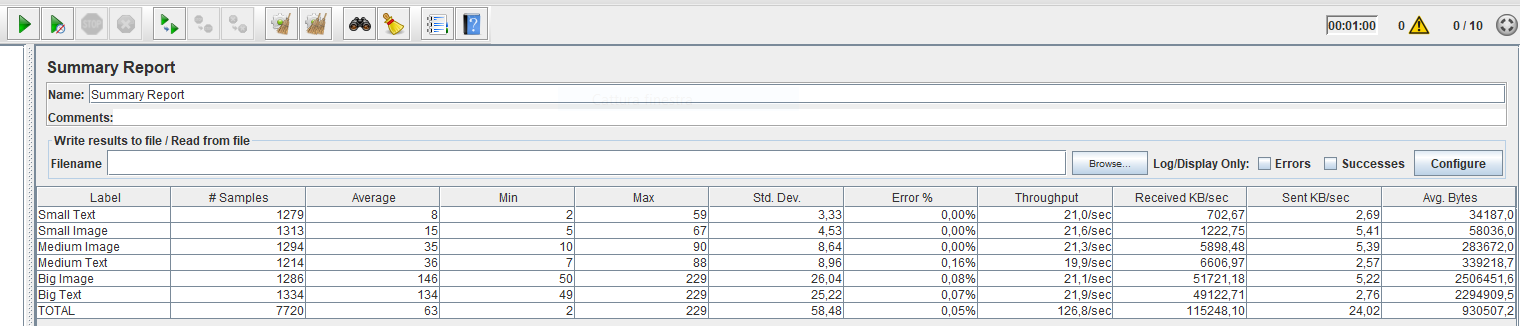
\includegraphics[width=\linewidth]{jmeter_analisi_10thread}
 		\end{figure}
 	\end{minipage}
 	\begin{minipage}{1\linewidth}
 		\begin{figure}[H]
 			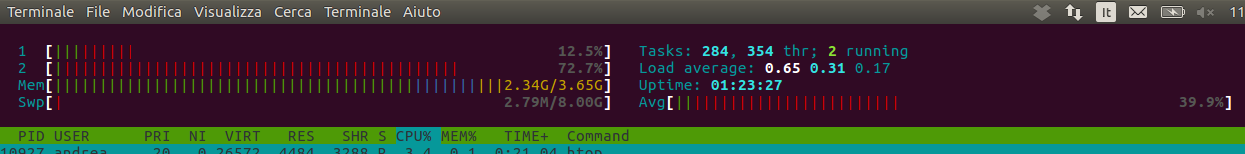
\includegraphics[width=\linewidth]{100_thread_server}
    \end{figure}
  \end{minipage}
\end{minipage}

\subsubsection{Esperimento con 100 Thread Group}
 \begin{minipage}{\linewidth}
 	\centering
 	\begin{minipage}{1\linewidth}
 		\begin{figure}[H]
 			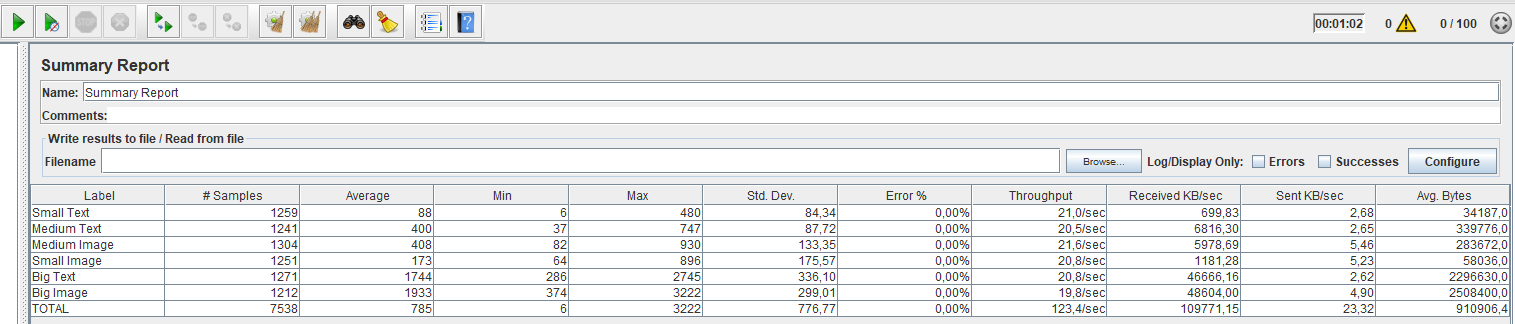
\includegraphics[width=\linewidth]{jmeter_analisi_100thread}
 		\end{figure}
 	\end{minipage}
 	\begin{minipage}{1\linewidth}
 		\begin{figure}[H]
 			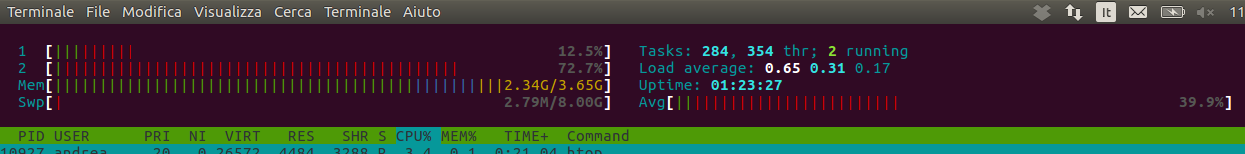
\includegraphics[width=\linewidth]{100_thread_server}
    \end{figure}
  \end{minipage}
\end{minipage}

\subsubsection{Esperimento con 500 Thread Group}
 \begin{minipage}{\linewidth}
 	\centering
 	\begin{minipage}{1\linewidth}
 		\begin{figure}[H]
 			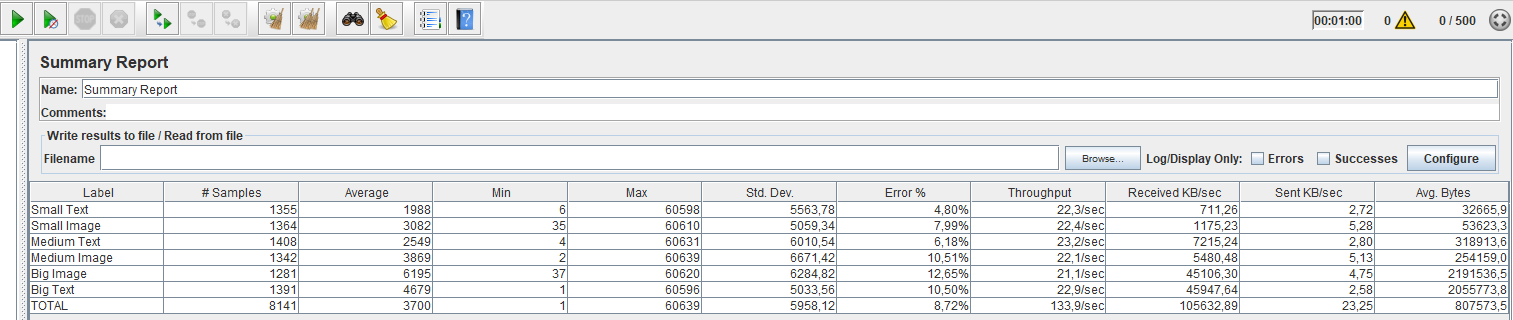
\includegraphics[width=\linewidth]{jmeter_analisi_500thread}
 		\end{figure}
 	\end{minipage}
 	\begin{minipage}{1\linewidth}
 		\begin{figure}[H]
 			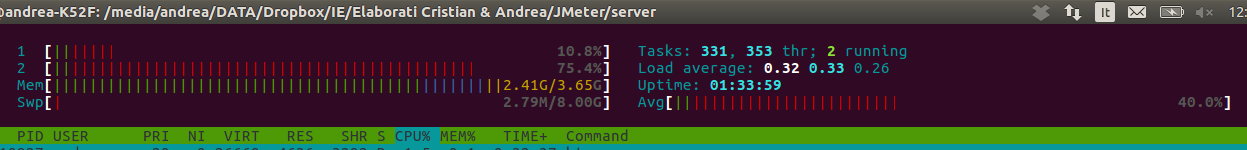
\includegraphics[width=\linewidth]{500_thread_server}
    \end{figure}
  \end{minipage}
\end{minipage}

\subsubsection{Esperimento con 1000 Thread Group}
 \begin{minipage}{\linewidth}
 	\centering
 	\begin{minipage}{1\linewidth}
 		\begin{figure}[H]
 			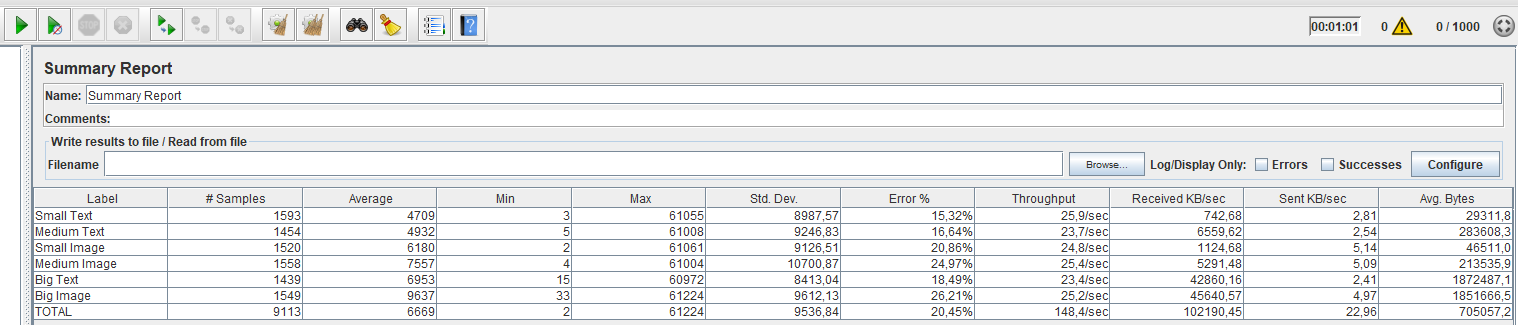
\includegraphics[width=\linewidth]{jmeter_analisi_1000thread}
 		\end{figure}
 	\end{minipage}
 	\begin{minipage}{1\linewidth}
 		\begin{figure}[H]
 			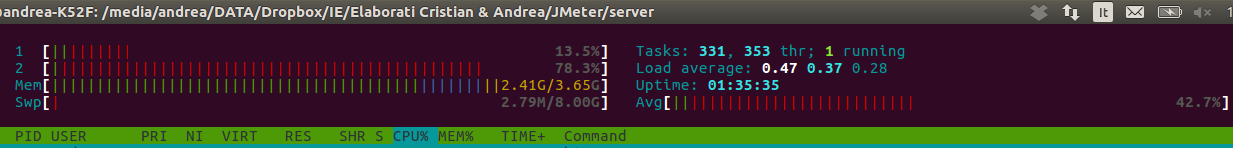
\includegraphics[width=\linewidth]{1000_thread_server}
    \end{figure}
  \end{minipage}
\end{minipage}

\vspace{1cm}
Il parametro Thread Group indica il numero di clients che effettuano continuamente
richieste HTTP al server.\\
Ovviamente questo numero di Threads è simulato dall'unica macchina client utilizzata,
tramite il tool JMeter.\\
Come si può osservare dalle immagini riportate, essendoci una sola macchina fisica,
al crescere del numero di richieste aumenta il numero di errori.\\
Questi errori però non sono da individuare nell'incapacità del server di gestire
la mole di richieste(infatti la CPU è mediamente occupata a circa il 40\% mentre
la RAM al 65\%), bensì nell'infrastruttura di rete(scheda di rete e cavo Ethernet),
limitata ad \textbf{1Gb/s}.\\

In \figurename~\ref{bottleneck_rete} è riportato l'utilizzo dell'I/O di rete,
raffigurante, in alcuni punti, il raggiungimento del limite fisico(1Gb/s).\\
\begin{figure}[!htbp]
  \centering
  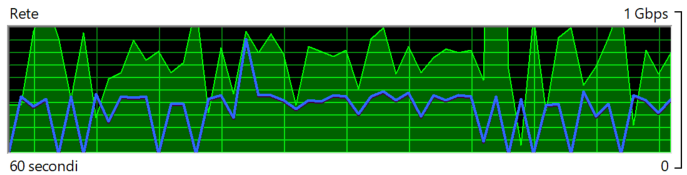
\includegraphics[width=1\linewidth, keepaspectratio]{client_rete_bottleneck}
  \caption{Infrastruttura di Rete - Bottleneck}
  \label{bottleneck_rete}
\end{figure}

\clearpage

\subsection{Analisi Alto Livello (Client)}
\subsubsection*{Impostazioni Client (JMeter)}
Prima di effettuare gli esperimenti, è stato necessario configurare alcuni parametri
nel Test Plan di JMeter, riportati in \figurename~\ref{conf_jmeter}

\begin{figure}[!htbp]
  \centering
  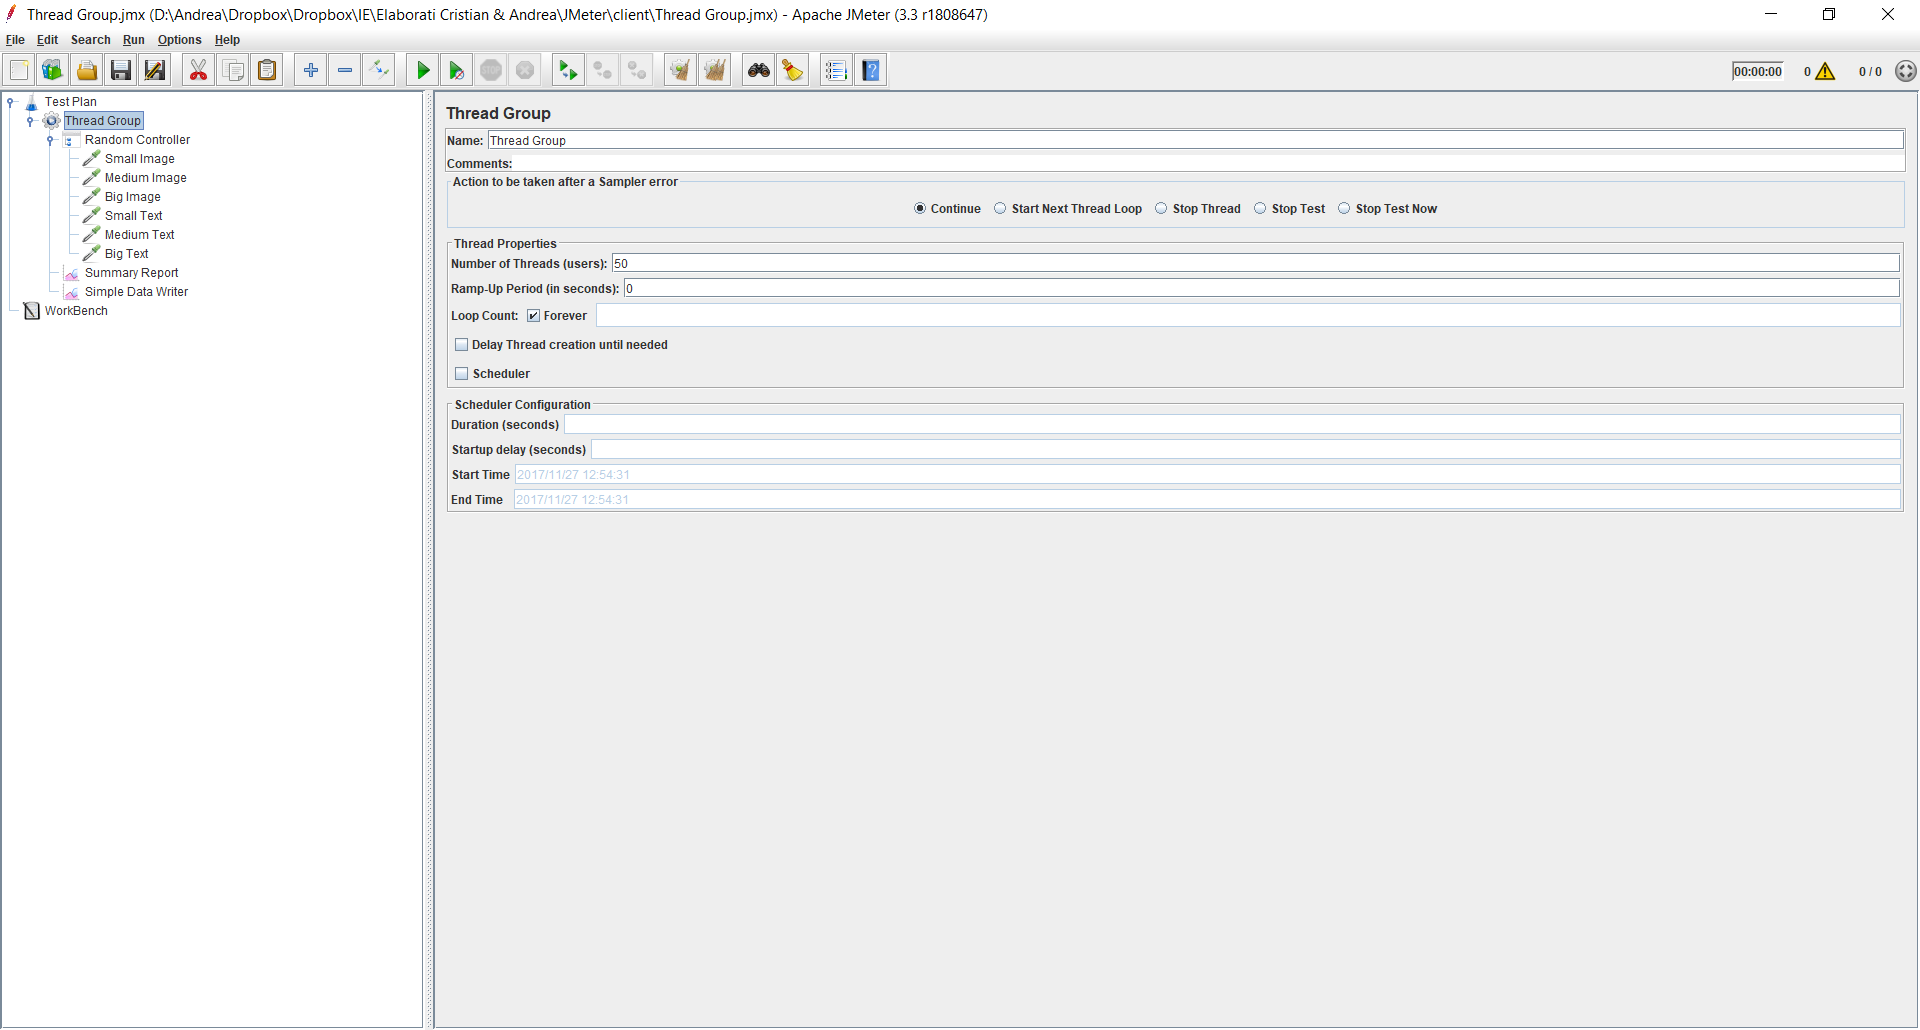
\includegraphics[width=1\linewidth, keepaspectratio]{conf_thread_group}
  \caption{}
  \label{conf_jmeter}
\end{figure}

In particolare, si evince che il Test Plan è stato caratterizzato dai seguenti
componenti:

\begin{itemize}
  \item \textbf{\textit{Random Controller}} - per generare richieste tra le possibili
  pagine in maniera randomica ed uniforme;
  \item \textbf{\textit{HTTP Request}} - una per pagina, serve per generare una
  richiesta HTTP;
  \item \textbf{\textit{Summary Report}} - genera un report immediato degli esperimenti
  in esecuzione.
  \item \textbf{\textit{Simple Data Writer}} - scrive i risultati degli esperimenti
  in un file .csv
\end{itemize}

JMeter è stato configurato attivando il \textbf{Keep Alive} ad ogni pagina
ed il parametro \textbf{Retrieve All Embedded Resources}(necessario per prelevare
le immagini linkate nell'html).\\
Nonostante gli esperimenti siano stati eseguiti per un tempo di 8 minuti, è stato
effettuato un filtraggio dei dati del primo ed ultimo minuto di esecuzione, al fine
di eliminare eventuali comportamenti transitivi.\\

I parametri utilizzati per la caratterizzazione del workload lato client sono:
\textbf{Latency}, \textbf{Elapsed Time}, \textbf{Bytes}.\\

In \figurename~\ref{distribuzioni_parametri} sono riportate le distribuzioni dei
tre parametri.\\

\begin{figure}[!htbp]
  \centering
  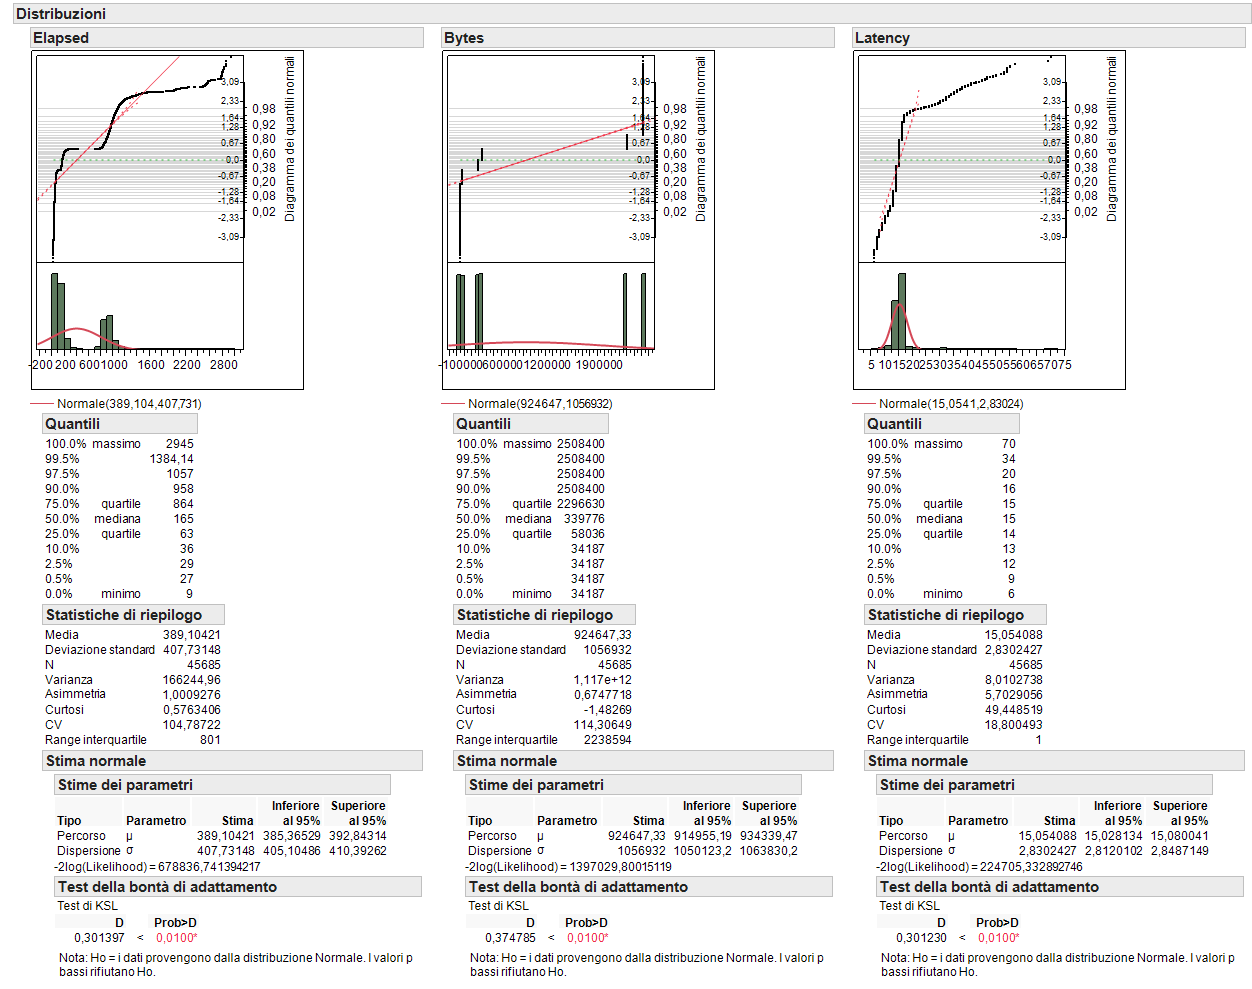
\includegraphics[width=1\linewidth, keepaspectratio]{distribuzioni_client}
  \caption{}
  \label{distribuzioni_parametri}
\end{figure}

Come si può osservare dal plot Q-Q e dal test di bontà di adattamento, le distribuzioni
non sono normali, di conseguenza, si scelgono \textit{mediana}, come indice di
tendenza centrale e \textit{SIQR}, come indice di dispersione.\\

\begin{center}
	\begin{tabular}{c|c|c|c|}
		& \textbf{Latency} & \textbf{Elapsed Time} & \textbf{Bytes} \\
		\hline
		\textbf{Mediana} & 15 & 165 & 339776 \\
		\hline
		\textbf{SIQR} & 1 & 801 & 2238594 \\
		\hline
	\end{tabular}
\end{center}

\subsubsection*{Correlazione Parametri}
Nella seguente fase vengono studiate possibili correlazioni presenti tra i tre
parametri considerati.\\
Per studiare la correlazione, non volendo fare assunzioni sulla natura delle
distribuzioni, è possibile svolgere il test non parametrico di \textbf{Kendall}.\\
Tale test assume come ipotesi nulla l'indipendenza dei fattori.\\
In particolare, si è interessati ad osservare eventuali correlazioni tra la Latency
e l'Elapsed Time, in \figurename~\ref{correlazione_elapsed_latency}.\\
\begin{figure}[!htbp]
  \centering
  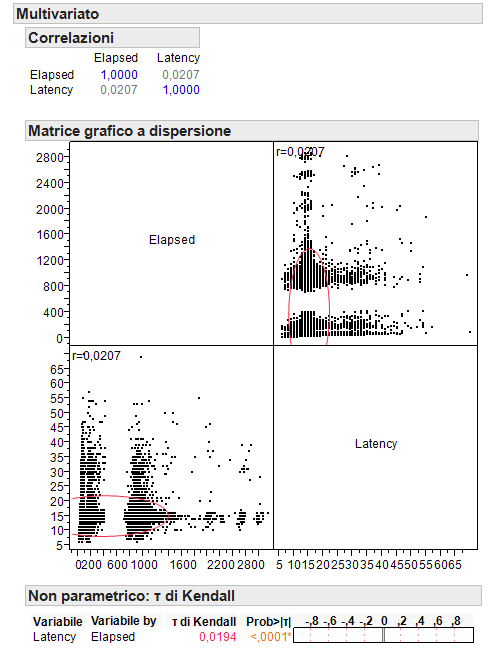
\includegraphics[width=.7\linewidth, keepaspectratio]{correlazione_elapsed_latency}
  \caption{Test di Kendall tra i parametri Elapsed Time e Latency}
  \label{correlazione_elapsed_latency}
\end{figure}

In questo caso, il test di Kendall suggerisce che l'ipotesi di indipendenza è
rigettata, quindi esiste una forte dipendenza tra i parametri \textit{Latency} e
\textit{Elapsed Time}.

\subsection{Analisi di basso livello: lato server}
Al fine di misurare il comportamento del server si è utilizzato il tool \textbf{collectl}
in concomitanza con l'avvio delle richieste del client.\\
Il comando lanciato nella bash linux è stato
``\textit{collectl -oT -scdmn -P --sep ,}", in particolare:

\begin{itemize}
  \item \textit{-oT}: aggiunge il timestamp;
  \item \textit{-scdmn}:  permette di selezionare la periferica di cui visualizzare
  i parametri e il dettaglio degli stessi;
  \item \textit{-P}: raggruppa i dati su singola riga;
  \item \textit{--sep ,}: aggiunge la vergola per la separazione dei dati;
\end{itemize}

La collectl effettua una misurazione ogni secondo, allo stesso modo del client sono
stati osservati 8 minuti e successivamente eliminati il primo e l'ultimo minuto.\\

Di seguito sono riportati i parametri considerati:
\begin{itemize}
  \item \textbf{CPU}:
  \begin{itemize}
    \item \textbf{\textit{Tot\%}}: percentuale di utilizzo della CPU ;
    \item \textbf{\textit{Idle\%}}: percentuale di idle della CPU;
    \item \textbf{\textit{Interpt/sec}}: numero di interrupt per secondo;
    \item \textbf{\textit{Ctx/sec}}: numero di contex switch per secondo.
  \end{itemize}
  \item \textbf{Disco}:
  \begin{itemize}
    \item \textbf{\textit{Reads}}: numero di letture al secondo;
    \item \textbf{\textit{RKBytes}}: KiloByte letti;
    \item \textbf{\textit{Writes}}: numero di scritture al secondo;
    \item \textbf{\textit{WKBytes}}: KiloByte scritti.
  \end{itemize}
  \item \textbf{RAM}:
  \begin{itemize}
    \item \textbf{\textit{Used}}: quantità di RAM fisica utilizzata;
    \item \textbf{\textit{Free}}: quantità di RAM fisica libera;
    \item \textbf{\textit{Buffered}}: quanti di RAM fisica utilizzata
   per bufferizzare file;
    \item \textbf{\textit{Cached}}: quantità di RAM fisica utilizzata come memoria cache;
    \item \textbf{\textit{Slab}}: quantità di memoria utilizzata dal kernel come cache per
    le strutture dati per utilizzo proprio;
    \item \textbf{\textit{Map}}: quantità di memoria che è stata utilizzata
   per mappare dispositivi, file o librerie utilizzando il comando mmap.
  \end{itemize}
  \item \textbf{Rete}
  \begin{itemize}
    \item \textbf{\textit{RxPkt}}: pacchetti inviati;
    \item \textbf{\textit{TxPkt}}: pacchetti trasmessi;
    \item \textbf{\textit{RxKB}}: KiloByte trasmessi;
    \item \textbf{\textit{TxKB}}: KiloByte inviati.
  \end{itemize}
\end{itemize}

Per caratterizzazione del workload sono state utilizzate le tecniche di  PCA e
clustering.
\clearpage
\subsubsection{PCA}
Prima di applicare la PCA sono stati analizzati gli andamenti temporali dei parametri,
la quale ha permesso l'eliminazione dei parametri riguardanti il disco, poichè
avendo eliminato il transitorio(primo ed ultimo minuto) il disco non effettuava
operazioni di lettura e/o scrittura causate della recezione o elaborazione di richieste http.
L'unico istante di tempo in cui il disco effettua una lettura è nell'inizio della sessione
di test, la quale però non è stata considerata per la caratterizzazione del workload.
Nella seguente figura è riportato il primo minuto di test, nel quale si osserva che all'inizio
c'è un picco di letture con una notevole crescita della memoria RAM utilizzata.


\begin{figure}[!htbp]
  \centering
  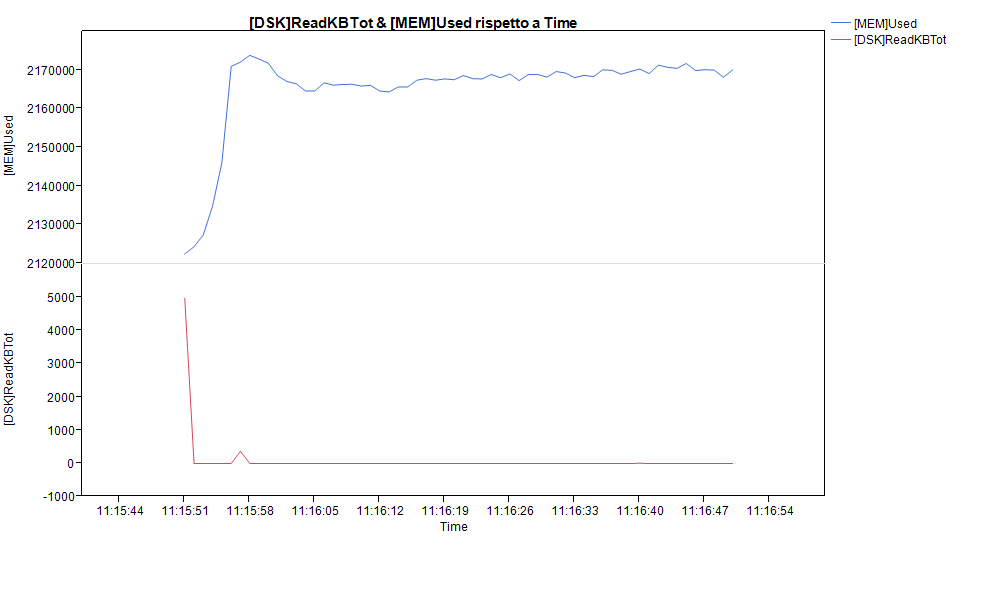
\includegraphics[width=\linewidth, keepaspectratio]{transitorio}
  \caption{Transitorio RAM/DISCO}
  \label{transitorio}
\end{figure}

\clearpage

Un'ulteriore analisi è stata fatta sul coefficiente
di variazione per poter trascurare sin da subito i parametri che hanno un CV nullo.\\
Di seguito è riportato il coefficiente di variazione per ogni parametro.\\

\begin{figure}[!htbp]
  \centering
  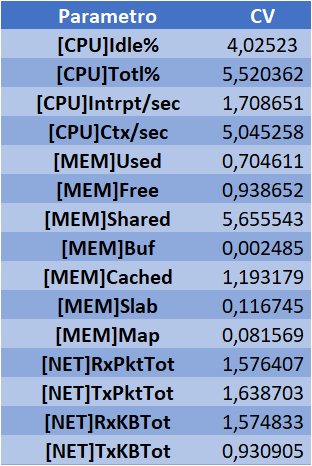
\includegraphics[width=.4\linewidth, keepaspectratio]{cv}
  \caption{CV parametri CPU e RAM}
  \label{cv1}
\end{figure}
\clearpage
Non è stato eliminato alcun parametro poichè non presentavano CV nullo, quindi è
stata applicata la PCA all'intero workload reale.\\
In figura è riportata il risultato ottenuto in JMP.\\

\begin{figure}[!htbp]
  \centering
  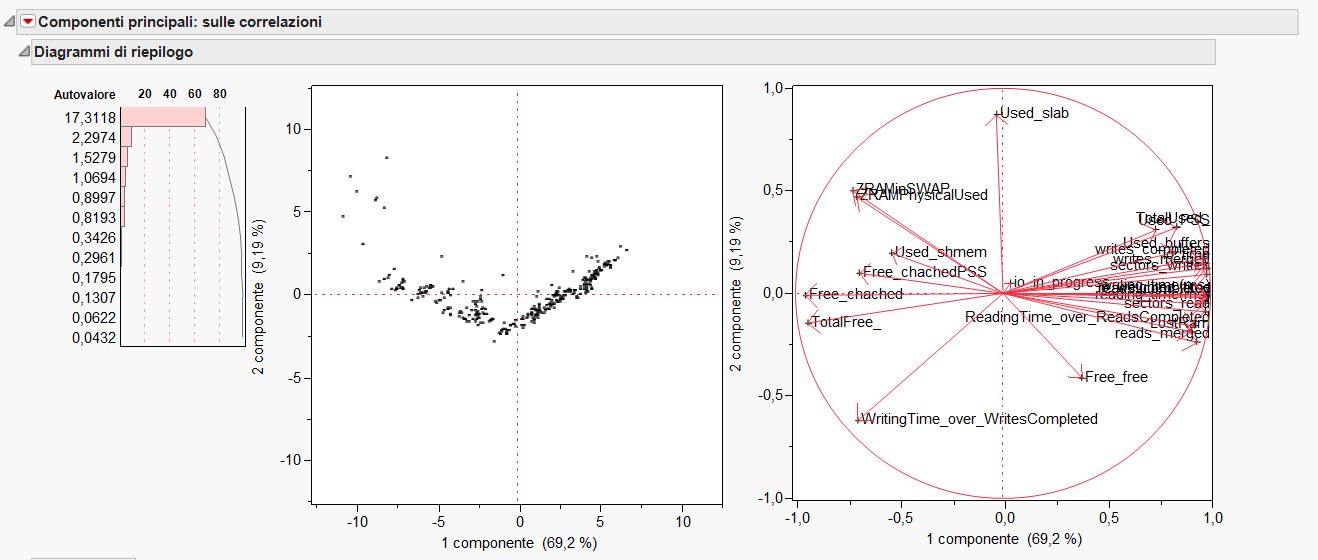
\includegraphics[width=1\linewidth, keepaspectratio]{pca}
  \caption{PCA}
  \label{pca}
\end{figure}

\begin{figure}[!htbp]
  \centering
  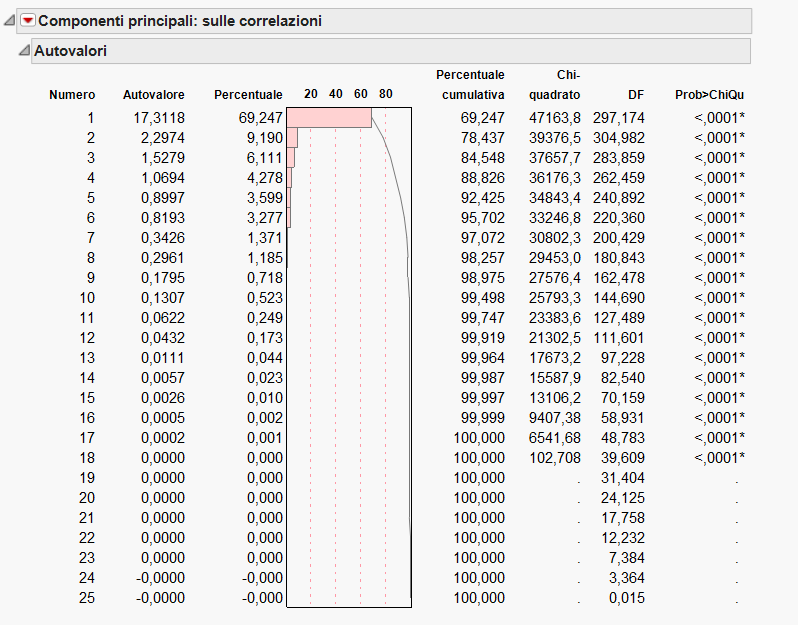
\includegraphics[width=1\linewidth, keepaspectratio]{autovalori}
  \caption{Autovalori PCA}
  \label{autovalori}
\end{figure}
\clearpage

\begin{figure}[!htbp]
  \centering
  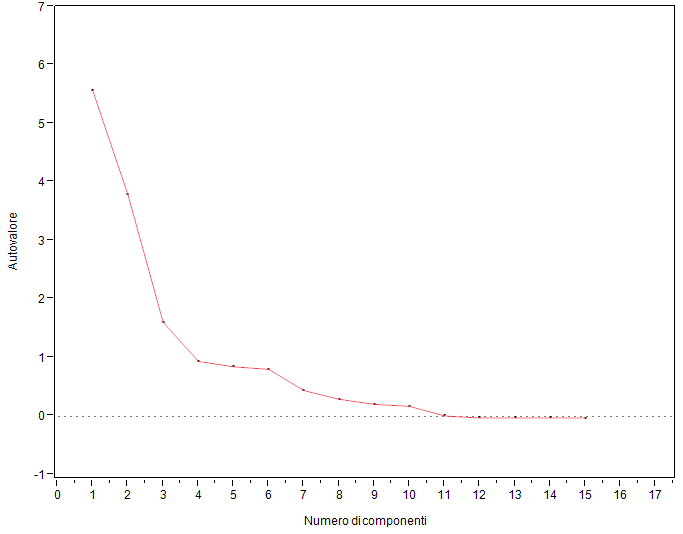
\includegraphics[width=.8\linewidth, keepaspectratio]{scree_pca}
  \caption{Grafico Scree}
  \label{scree_pca}
\end{figure}

Osservando le figure \ref{autovalori} e \ref{scree_pca} si è scelto di considerare
7 componenti principali conservando il 94,680\% di varianza.
\clearpage
\subsubsection{Clustering}

Dopo aver scelto il numero di componenti è stato applicato l clustering per poter
ridurre il numero di righe del workload reale.\\
In figura è riportato il dentogramma risultante dal clustering gerarchico con
la relativa curva di clustering ottenuta in JMP.\\

\begin{figure}[!htbp]
  \centering
  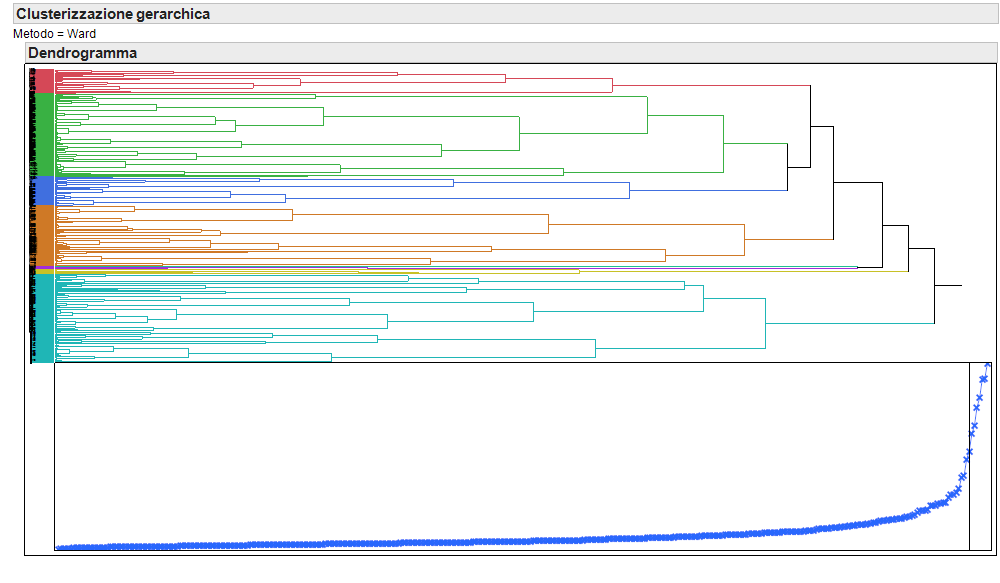
\includegraphics[width=1\linewidth, keepaspectratio]{clustering}
  \caption{Clustering}
  \label{clustering}
\end{figure}
\clearpage

Osservando le figure \ref{clustering}, \ref{gerarchia_cluster} e \ref{ccc}
il numero di cluster scelti è 8, poichè aggiungendo un ulteriore cluster il guadagno
in termini varianza conservata è trascurabile.

\begin{minipage}{\linewidth}
 \centering
 \begin{minipage}{0.48\linewidth}
   \begin{figure}[H]
     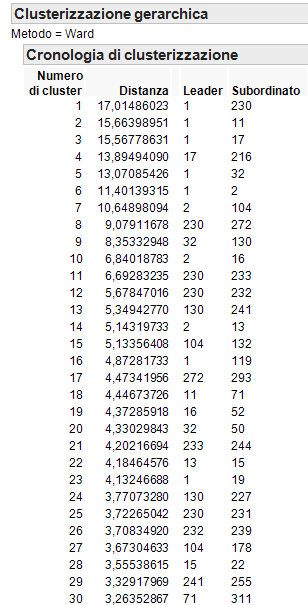
\includegraphics[width=0.9\linewidth]{gerarchia_cluster}
     \label{gerarchia_cluster}
     \caption{Gerarchia di clustering}
   \end{figure}
 \end{minipage}
 \begin{minipage}{0.48\linewidth}
   \begin{figure}[H]
     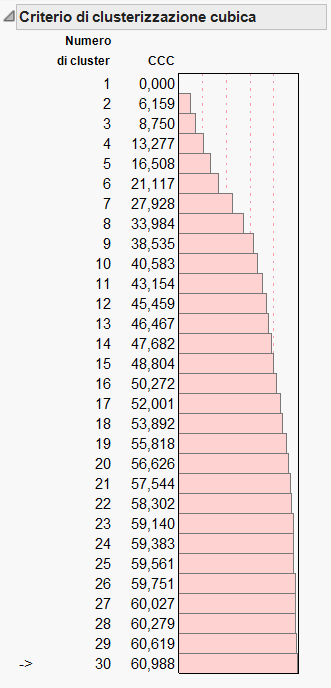
\includegraphics[width=.9\linewidth]{ccc}
     \label{ccc}
     \caption{Criterio di Clusterizzazione Cubica}
   \end{figure}
 \end{minipage}
\end{minipage}

Osservando le figure \ref{clustering}, \ref{gerarchia_cluster} e \ref{ccc} si è
scelto di considerare 8 cluster.
\clearpage
\subsubsection{Caratterizzazione Cluster}

Per caratterizzare ogni cluster, ovvero per individuare quale stato del sistema
rappresenta ogni cluster, sono state analizzate le figure \ref{autovettori}, \ref{graph}
e \ref{cluster_time}.\\
La figura \ref{autovettori} mostra gli autovettori delle 7 componenti principali
dalle quali si individuazione da quali parametri del workload reale esse sono state influenzate.\\
\begin{figure}[!htbp]
  \centering
  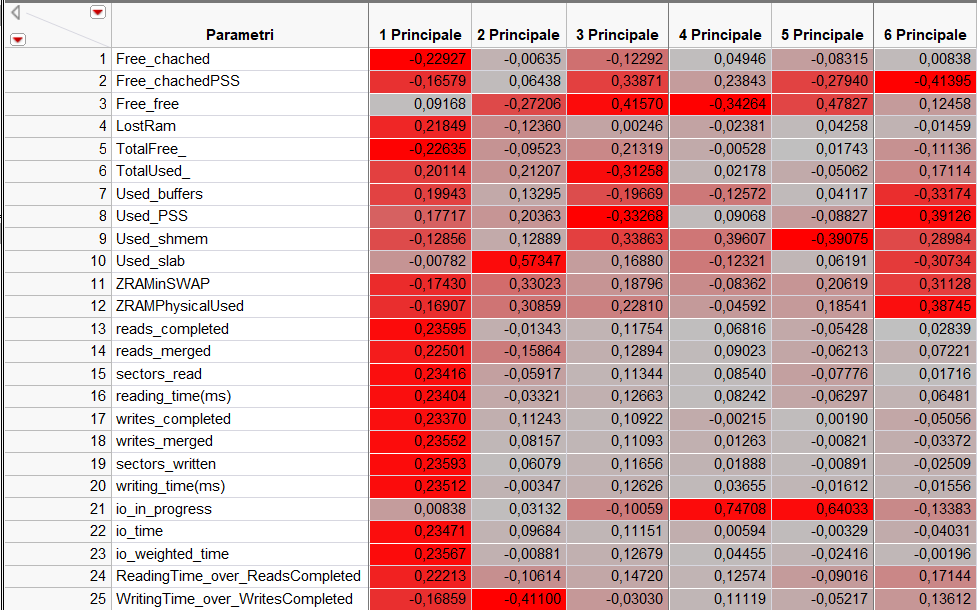
\includegraphics[width=.9\linewidth, keepaspectratio]{autovettori}
  \caption{Autovettori PCA}
  \label{autovettori}
\end{figure}

Dalla figura \ref{autovettori} si evidenzia il significato delle singole componenti
principali, in particolare:

\begin{itemize}
  \item \textbf{\textit{Principale 1}}: influenzata maggiormente di parametri che
  riguardano la RAM.\\
  Nello specifico si nota che \textit{Used} e \textit{Free} si comportano in maniera duale;
  \item \textbf{\textit{Principale 2}}: influenzata maggiormente dai parametri
  di rete, \textit{Intrpt/sec} e \textit{Idle\%};
  \item \textbf{\textit{Principale 3}}: influenzata da \textit{Totl\%} e \textit{Idle\%};
  \item \textbf{\textit{Principale 4}}: influenzata da \textit{Map} e \textit{TxPktTot};
  \item \textbf{\textit{Principale 5}}: influenzata da \textit{Ctx/sec} e \textit{TxPktTot};
  \item \textbf{\textit{Principale 6}}: influenzata da \textit{Ctx/sec}, \textit{Map},
  \textit{RxPktTot}, \textit{TxPktTot} e \textit{RxKBTot};
  \item \textbf{\textit{Principale 7}}: \textit{Buf} e \textit{Slab};
\end{itemize}

\clearpage

La figura \ref{graph} mostra quali sono le componenti principali che hanno contribuito
maggiormente alla creazione dei cluster.\\

\begin{figure}[!htbp]
  \centering
  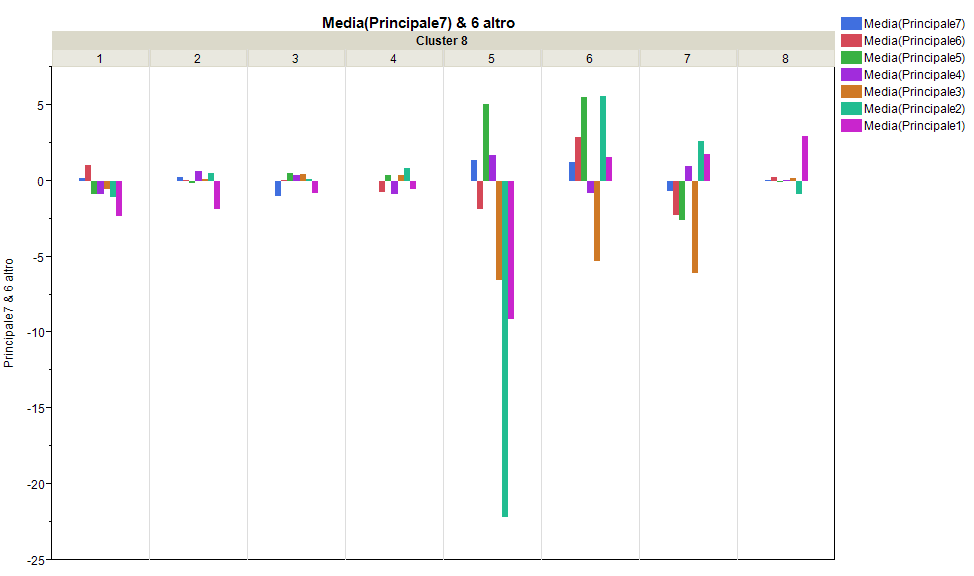
\includegraphics[width=0.8\linewidth, keepaspectratio]{graph}
  \caption{}
  \label{graph}
\end{figure}
La figura \ref{cluster_time} mostra la composizione dei cluster rispetto al tempo.\\
\begin{figure}[!htbp]
  \centering
  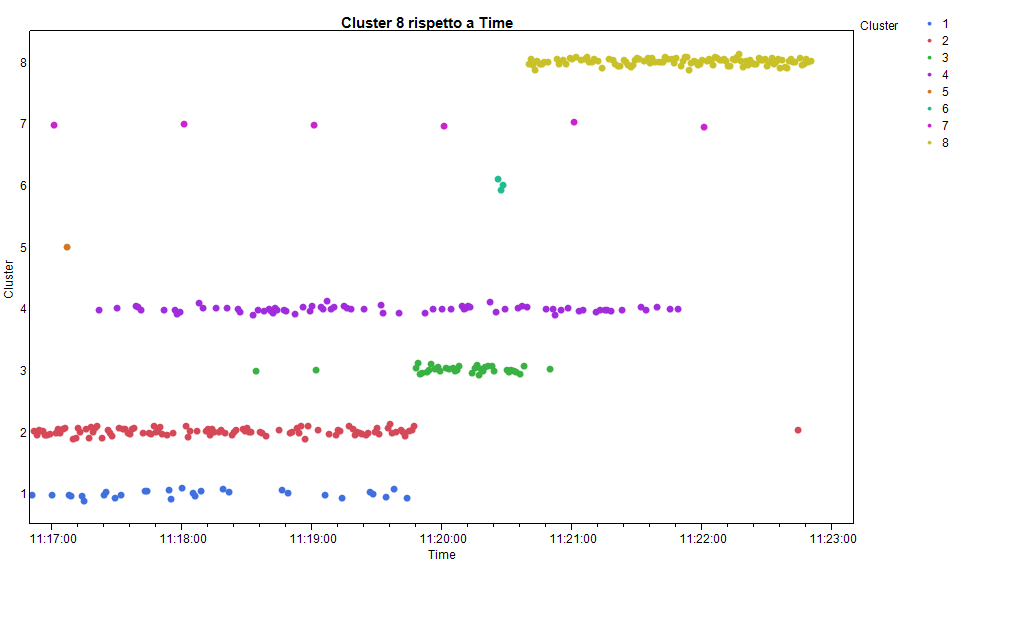
\includegraphics[width=.8\linewidth, keepaspectratio]{cluster_time}
  \caption{}
  \label{cluster_time}
\end{figure}

\clearpage

Di seguito è riportata la caratterizzazione dei singoli cluster ed una rappresentazione
grafica 3D nella quale la sfumatura dei campioni plottati va dal blu al rosso, dove
il blu rappresenta il primo minuto e il rosso l'ultimo.

\begin{itemize}

  \begin{figure}[!htbp]
    \centering
    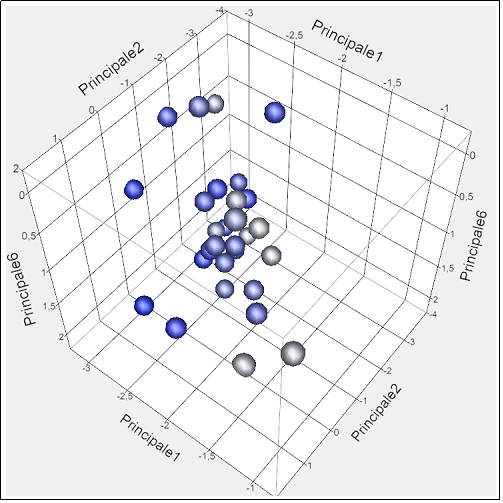
\includegraphics[width=.45\linewidth, keepaspectratio]{cluster1}
    \caption{Grafico 3D del Cluster 1}
    \label{cluster1}
  \end{figure}

  \item \textbf{Cluster 1}: influenzato maggiormente da valori negativi della
  prima e seconda componente principale e positivi della sesta.\\
  In particolare, osservando la figura \ref{cluster_time} e \ref{cluster1}, i campioni contenuti
  in questo cluster appartengono alla prima metà dell'esperimento.\\
  Analizzando più approfonditamente la cause della creazione di tale cluster si
  identifica quale stato del sistema esso rappresenta.\\
  A causa di valori negativi della prima componente principale esso
  rappresenta uno stato del sistema con memoria RAM occupata in bassa quantità,
  in quanto il valore della parametro \textit{Free} nei campioni del cluster 1,
  essendo negativo in corrispondenza della principale uno in figura \ref{autovettori},
  è sicuramente maggiore rispetto agli altri parametri, in particolare memoria RAM.\\
  Inoltre si può affermare che a causa della seconda componente principale negativa
  l'attività di rete è bassa, in quanto nella figura \ref{autovettori} si osserva
  che i parametri di reti influenzano positivamente la principale due, dunque
  per assumere valori negativi i parametri di rete devono assumere valori bassi.

  \clearpage

  \begin{figure}[!htbp]
    \centering
    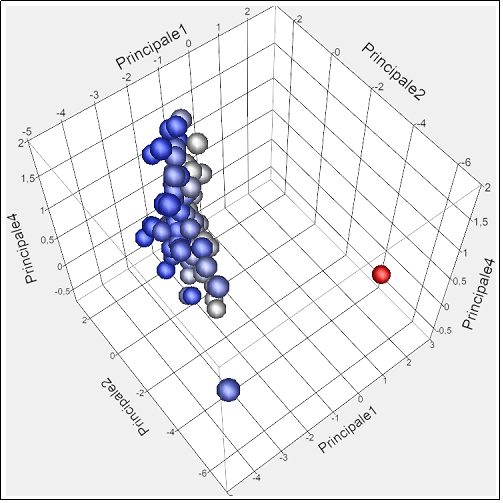
\includegraphics[width=.45\linewidth, keepaspectratio]{cluster2}
    \caption{Cluster 2}
    \label{cluster2}
  \end{figure}

  \item \textbf{Cluster 2}: influenzato maggiormente da valori negativi della
  prima e positivi seconda e quarta componente principale.\\
  In particolare, osservando la figura \ref{cluster_time} e \ref{cluster1}, i campioni contenuti
  in questo cluster appartengono alla prima metà dell'esperimento.\\
  Analizzando più approfonditamente la cause della creazione di tale cluster si
  identifica quale stato del sistema esso rappresenta.\\
  In particolare il cluster rappresenta uno stato in cui la quantità di RAM occupata
  è bassa, comportamento verificato nel primo cluster, ma in maniera opposta,
  essendo positiva la principale 2 presenta un'attività di rete più intensa.

  \clearpage

  \begin{figure}[!htbp]
    \centering
    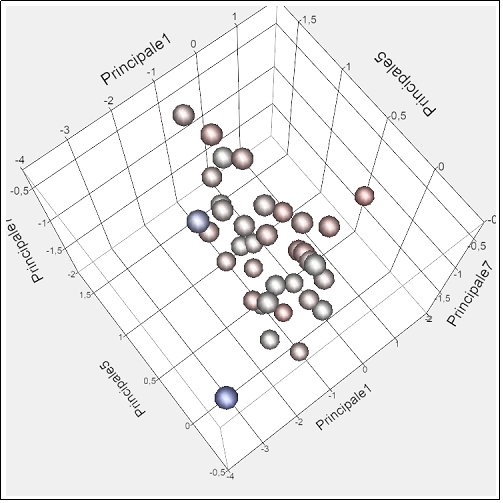
\includegraphics[width=0.45\linewidth, keepaspectratio]{cluster3}
    \caption{Cluster 3}
    \label{cluster3}
  \end{figure}

  \item \textbf{Cluster 3}: influenzato maggiormente da valori negativi della
  prima e settima principale, e positivi della quinta.
  In particolare, osservando la figura \ref{cluster_time} e \ref{cluster1}, i campioni contenuti
  in questo cluster appartengono ad un intervallo temporale centrale dell'esperimento.\\
  Analizzando più approfonditamente la cause della creazione di tale cluster si
  identifica quale stato del sistema esso rappresenta.\\
  In particolare il cluster rappresenta uno stato in cui la quantità di RAM occupata
  è bassa, comportamento verificato nel primo cluster, con attivata di rete in trasmissione
  bassa e aumento delle memoria RAM dedicato al buffering dei file;

  \clearpage

  \begin{figure}[!htbp]
    \centering
    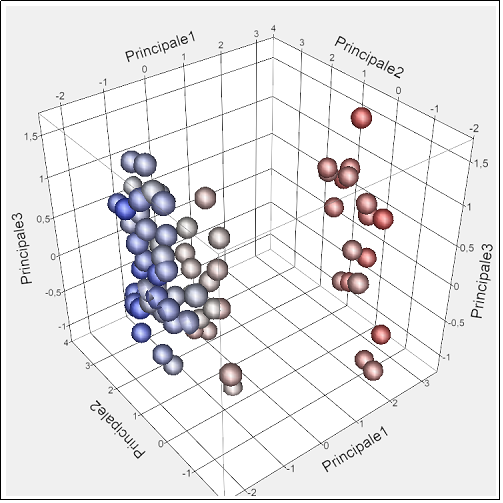
\includegraphics[width=.45\linewidth, keepaspectratio]{cluster4}
    \caption{Cluster 4}
    \label{cluster4}
  \end{figure}

  \item \textbf{Cluster 4}: presenta valori componenti principale per cui non
  rende possibile una caratterizzazione corretta, quindi per poterlo analizzare
  si è suddiviso il cluster in due sotto-cluster utilizzando la cronologia di
  clusterizzazione mostrata precedentemente, in figura \ref{cluster_4_diviso} è
  riportata l'incidenza delle componenti principali sui due sotto-cluster.\\

  \begin{figure}[!htbp]
    \centering
    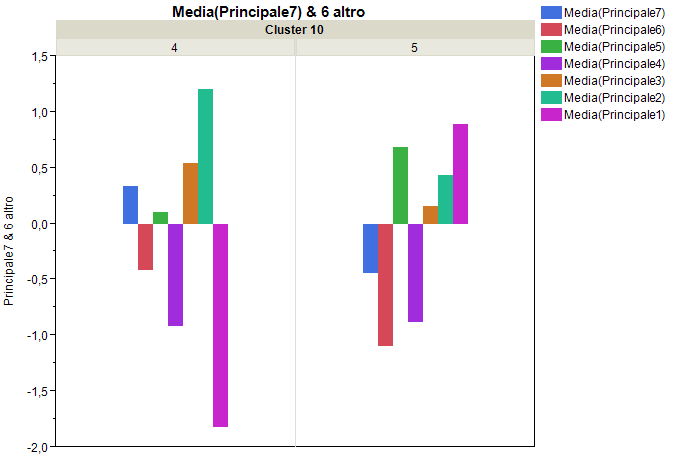
\includegraphics[width=.6\linewidth, keepaspectratio]{cluster_4_diviso}
    \caption{}
    \label{cluster_4_diviso}
  \end{figure}

  Dalla figura \ref{cluster_4_diviso} si possono caratterizzare i cluster 4.1 e 4.2.\\
  Il cluster 4.1 risulta influenzato  negativamente delle principali uno e quattro
  e positivamente dalla principale 2, quindi c'è un alta attività di rete
  e una bassa quantità di memoria RAM occupata.\\
  Il cluster 4.2 risulta influenzato negativamente delle principali sei e quattro,
  e positivamente dalla principale 1.\\
  Dunque si evince un'alta attività di rete e un'alta quantità di memoria RAM occupata.

  \begin{figure}[!htbp]
    \centering
    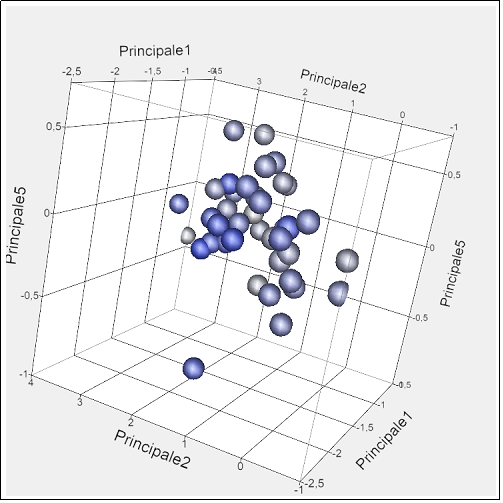
\includegraphics[width=.45\linewidth, keepaspectratio]{cluster41}
    \caption{Cluster 4.1}
    \label{cluster41}
  \end{figure}

  \begin{figure}[!htbp]
    \centering
    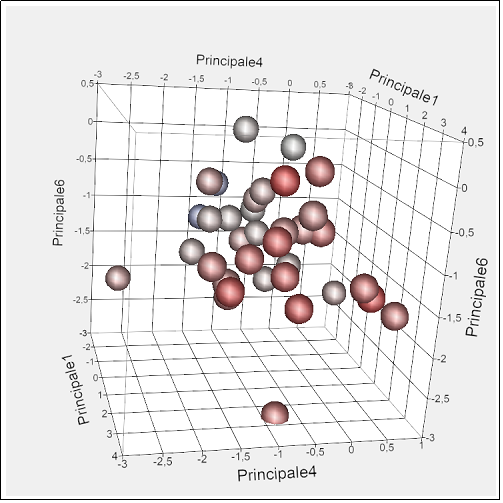
\includegraphics[width=.45\linewidth, keepaspectratio]{cluster42}
    \caption{Cluster 4.2}
    \label{cluster42}
  \end{figure}

  \clearpage

  \begin{figure}[!htbp]
    \centering
    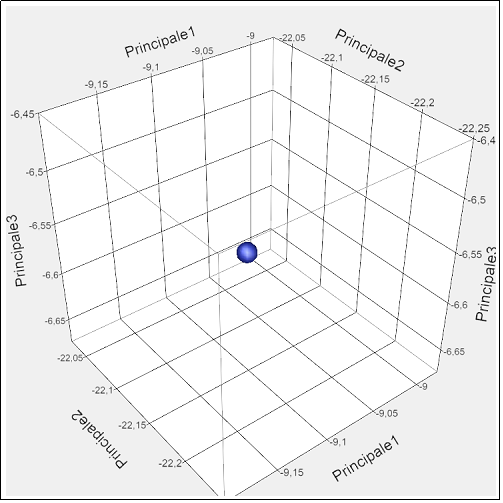
\includegraphics[width=.45\linewidth, keepaspectratio]{cluster5}
    \caption{Cluster 5}
    \label{cluster5}
  \end{figure}

  \item \textbf{Cluster 5}: tale cluster è formato da un solo campione, essendo
  esso un outlier va analizzato per capire se può essere eliminato.\\
  La creazione di tale cluster è attribuita maggiormente dalla principale
  due la quale è stata condizionata maggiormente dai parametri \textbf{RxPktTot}
  e \textbf{RxKBTot}.\\
  Analizzando il grafico in figura \ref{cluster5_temp_analisi}, il quale riporta
  l'andamento temporale di \textbf{RxKBTot}, si osserva che in corrispondenza del
  cluster 5 c'è un picco negativo il quale può essere attribuito ad una riduzione
  della velocità di trasmissione del client, quindi il tale cluster non sarà
  considerato per la generazione del workload sintetico.\\

  \begin{figure}[!htbp]
    \centering
    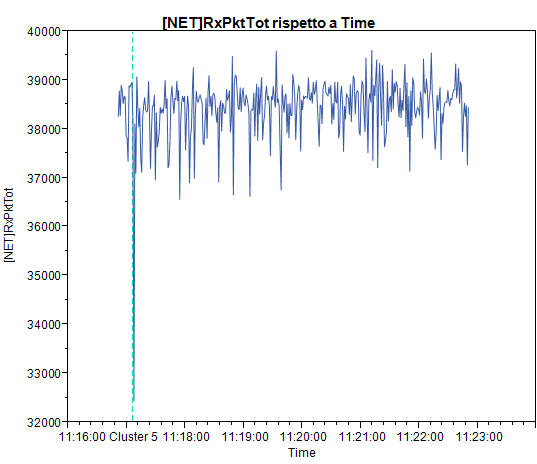
\includegraphics[width=.5\linewidth, keepaspectratio]{cluster5_temp_analisi}
    \caption{Andamento temporale di RxPktTot}
    \label{cluster5_temp_analisi}
  \end{figure}

  \clearpage

  \begin{figure}[!htbp]
    \centering
    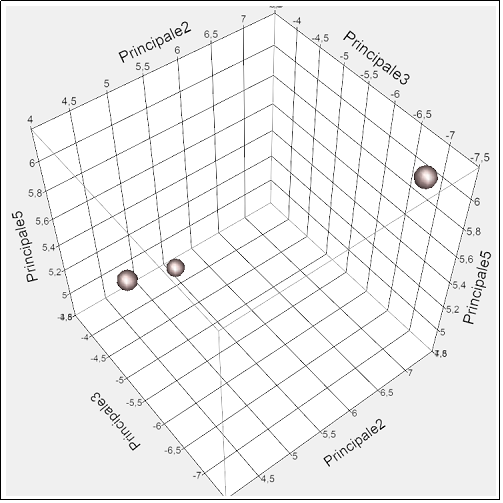
\includegraphics[width=0.45\linewidth, keepaspectratio]{cluster6}
    \caption{Cluster 6}
    \label{cluster6}
  \end{figure}

  \item \textbf{Cluster 6}: la formazione di tale cluster è attribuita alle
  componenti principali 2,3 e 5, le quali sono state influenzate maggiormente
  da \textit{RxPktTot}, \textit{Tot\%}, \textit{TxPktTot} e \textit{Ctx/s}.\\
  Analizzando la figura \ref{analisi_temp_cluster_6}, la quale riporta l'andamento
  temporale dei parametri sopra descritti, si nota che tali campioni sono consecutivi
  e che individuano un picco di \textit{Ctx/s} il quale può essere attributo all'esecuzione
  di altri processi presenti nel server in quanto sul server sono in esecuzioni
  diversi processi, quindi si può ritenere irrilevante tale cluster al fine
  della caratterizzazione del workload.\\

  \begin{figure}[!htbp]
    \centering
    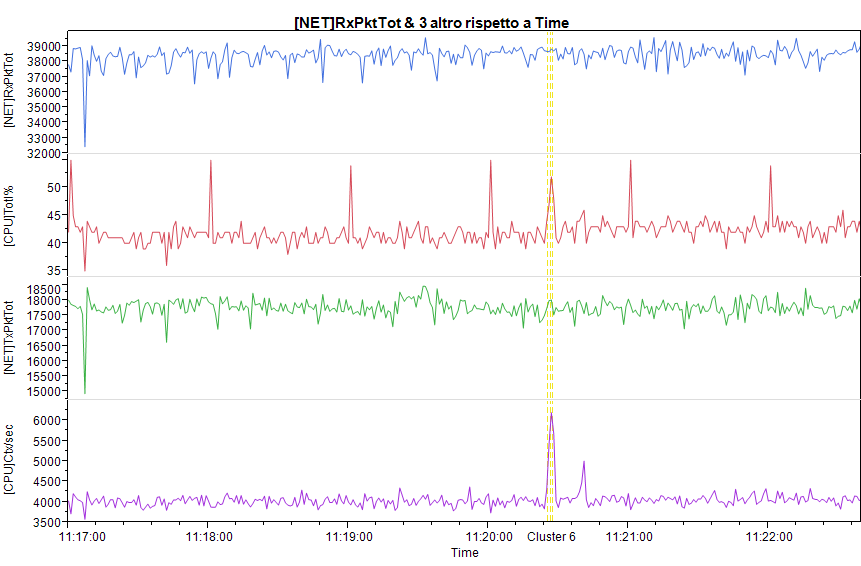
\includegraphics[width=0.6\linewidth, keepaspectratio]{analisi_temp_cluster_6}
    \caption{Analisi temporale \textit{RxPktTot}, \textit{Tot\%}, \textit{TxPktTot} e \textit{Ctx/s}}
    \label{analisi_temp_cluster_6}
  \end{figure}

  \clearpage

  \begin{figure}[!htbp]
    \centering
    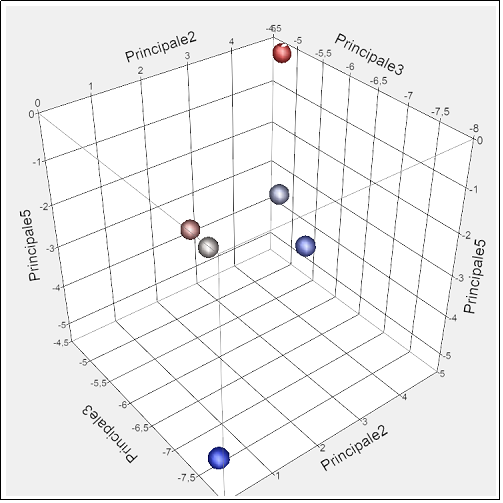
\includegraphics[width=.45\linewidth, keepaspectratio]{cluster7}
    \caption{Cluster 7}
    \label{cluster7}
  \end{figure}

  \item \textbf{Cluster 7}: la formazione di tale cluster è attribuibile maggiormente
  alla terza componente principale, la quale è stata influenza dal parametro \textit{Tot\%}.
  Analizzando il comportamento temporale di tale parametro, in figura \ref{analisi_temp_cluster_7},
  si osserva che tale cluster contiene picchi di utilizzo della CPU, in particolare
  essi si verificano ogni primo secondo.\\
  Tale comportamento può essere attribuito al sistema operativo, quindi non sarà
  considerato per creazione del workload sintetico.

  \begin{figure}[!htbp]
    \centering
    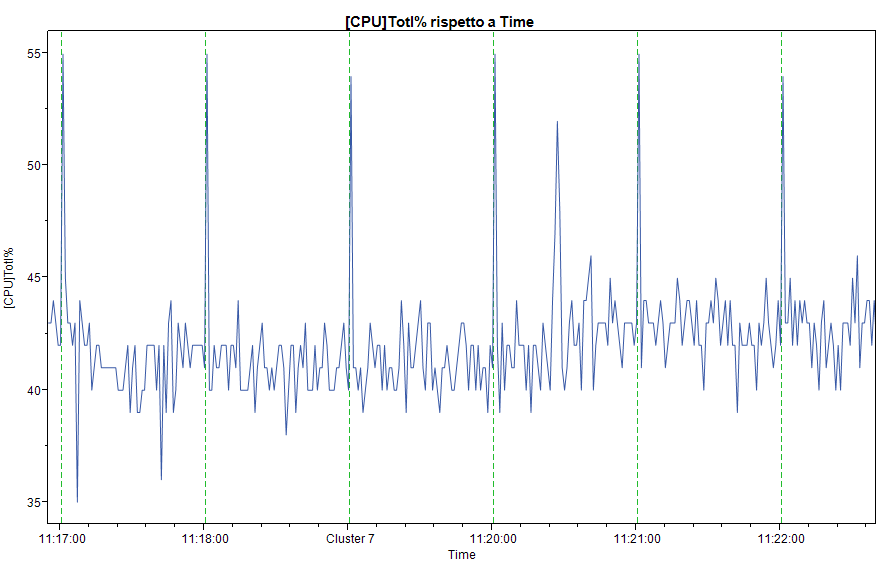
\includegraphics[width=0.6\linewidth, keepaspectratio]{analisi_temp_cluster_7}
    \caption{Analisi temporale \textit{Tot\%}}
    \label{analisi_temp_cluster_7}
  \end{figure}

  \clearpage

  \begin{figure}[!htbp]
    \centering
    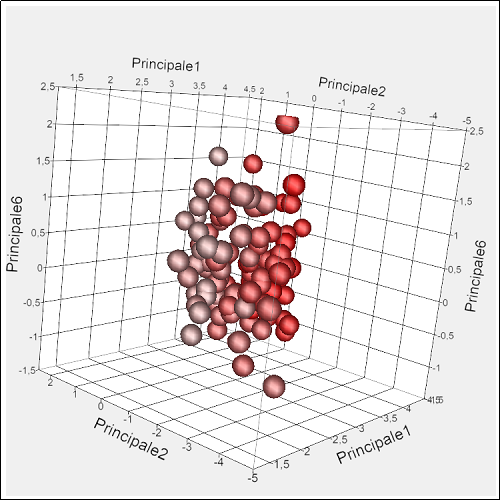
\includegraphics[width=.45\linewidth, keepaspectratio]{cluster8}
    \caption{Cluster 8}
    \label{cluster8}
  \end{figure}

  \item \textbf{Cluster 8}: rappresenta la parte finale dell'esperimento.\\
   Dunque lo stato del sistema che esso rappresenta è dato da valori di RAM occupata elevati
   e una bassa attività di rete.\\
   In pratica risulta essere il duale del \textit{cluster 1}.\\

\end{itemize}
  \clearpage
Scegliendo come punti rappresentanti di ogni cluster il centroide il Workload
ottenuto è il seguente.
\begin{figure}[!htbp]
  \centering
  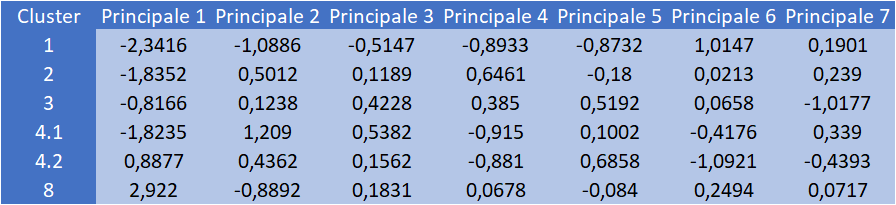
\includegraphics[width=1\linewidth, keepaspectratio]{centroidi}
  \caption{Workload Sintetico}
  \label{centroidi}
\end{figure}

La percentuale di devianza persa approssimando il workload reale con il workload
sintetico è il 33,27\%.

\begin{minipage}{\linewidth}
 \centering
 \begin{minipage}{0.48\linewidth}
   \begin{figure}[H]
     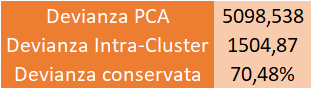
\includegraphics[width=0.9\linewidth]{devianza}
   \end{figure}
 \end{minipage}
 \begin{minipage}{0.48\linewidth}
   \begin{figure}[H]
     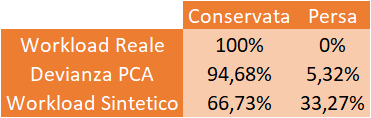
\includegraphics[width=.9\linewidth]{significativita_workload}
   \end{figure}
 \end{minipage}
\end{minipage}

\section{Capacity Test}
Questa sezione è dedicata allo studio della capacità di carico del sistema.\\
Il capacity test è attuato sulla base del workload caratterizzato in precedenza,
in funzione della tipologia di richieste effettuate al server(pagine di
piccola, media e grande dimensione).\\
I parametri di interesse nel capacity test sono le \textit{Richieste al minuto(Req/min)},
il \textit{Throughput} e l'\textit{Elapsed Time}.\\
Il test procede incrementando le Req/min ed osservando i 2 parametri di risposta
del sistema.\\
Plottando i risultati ottenuti è possibile individuare due punti di funzionamento
del sistema, noti come:
\begin{itemize}
  \item \textbf{Knee Capacity} - punto di funzionamento in cui il sistema ha un
  buon throughput e dei tempi di risposta bassi;
  \item \textbf{Usable Capacity} - punto di funzionamento limite in cui il sistema
  ha un ottimo throughput, ma oltre il quale c'è un degrado notevole nelle prestazioni.
\end{itemize}

Per il test effettuato con il tool JMeter, è stato scelto di di simulare 50 Threads
attivi.\\

\subsection{Test pagine HTML piccole}
In questo caso sono state utilizzate esclusivamente le richieste HTTP per le pagine
\textit{small\_text} e \textit{small\_image}.\\
In \figurename~\ref{small_page_summary_report} sono presenti gli esiti del
Summary Report di JMeter.\\

\begin{figure}[!htbp]
  \centering
  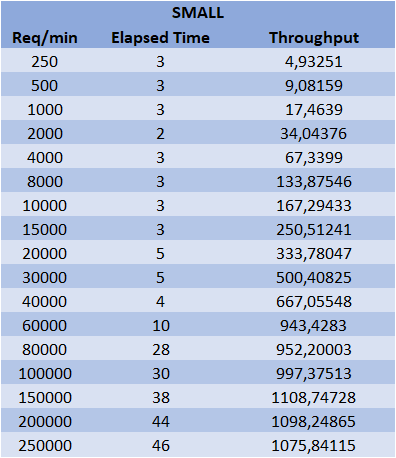
\includegraphics[width=.4\linewidth, keepaspectratio]{capacitytest_small}
  \caption{Test pagine HTML piccole}
  \label{small_page_summary_report}
\end{figure}

Utilizzando il costruttore di Grafici di \textit{JMP} sono stati analizzati i plot
di Throughput ed Elapsed Time, e definiti i punti di \textit{Knee Capacity} e
\textit{Usable Capacity}.\\

\begin{figure}[!htbp]
  \centering
  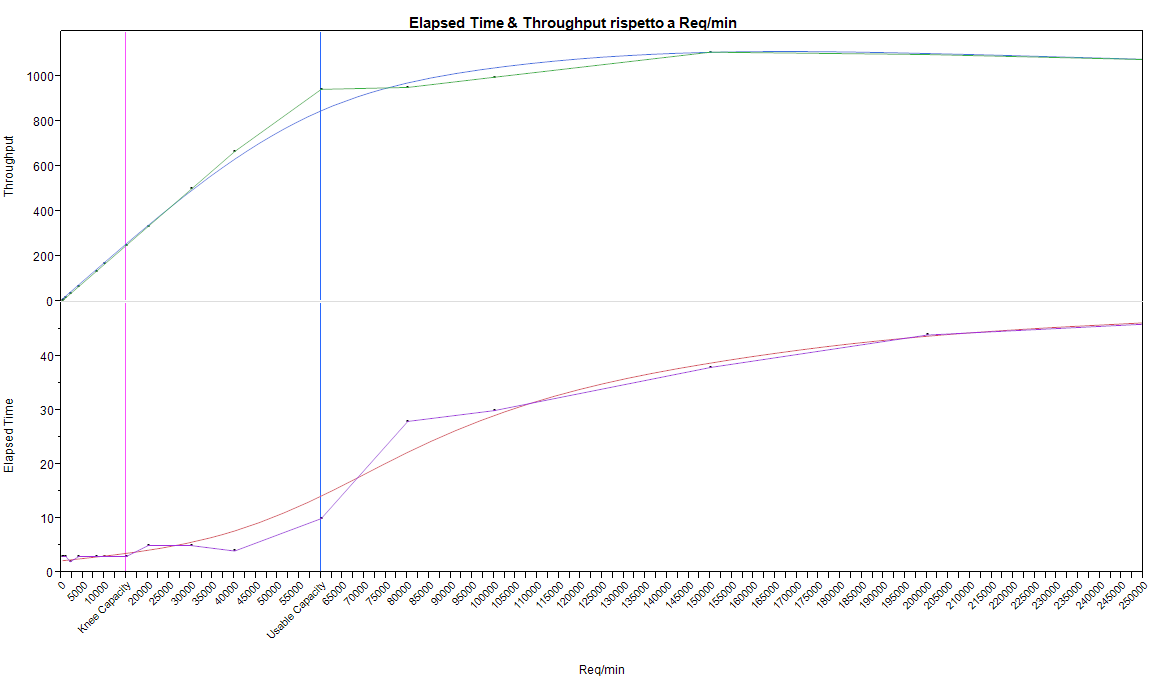
\includegraphics[width=\linewidth, keepaspectratio]{usable_knee_small}
  \caption{Capacity: Knee (15000 Req/min) / Usable (60000 Req/min)}
\end{figure}

\subsection{Test pagine HTML medie}
In questo caso sono state utilizzate esclusivamente le richieste HTTP per le pagine
\textit{medium\_text} e \textit{medium\_image}.\\
In \figurename~\ref{medium_page_summary_report} sono presenti gli esiti del
Summary Report di JMeter.\\

\begin{figure}[!htbp]
  \centering
  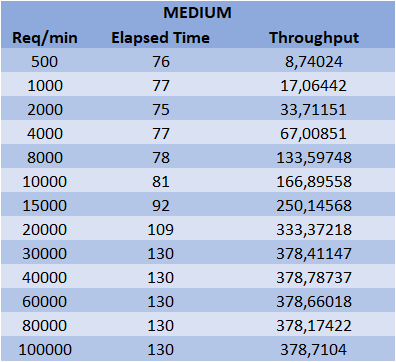
\includegraphics[width=.4\linewidth, keepaspectratio]{capacitytest_medium}
  \caption{Test pagine HTML medie}
  \label{medium_page_summary_report}
\end{figure}

Utilizzando il costruttore di Grafici di \textit{JMP} sono stati analizzati i plot
di Throughput ed Elapsed Time, e definiti i punti di \textit{Knee Capacity} e
\textit{Usable Capacity}.\\

\begin{figure}[!htbp]
  \centering
  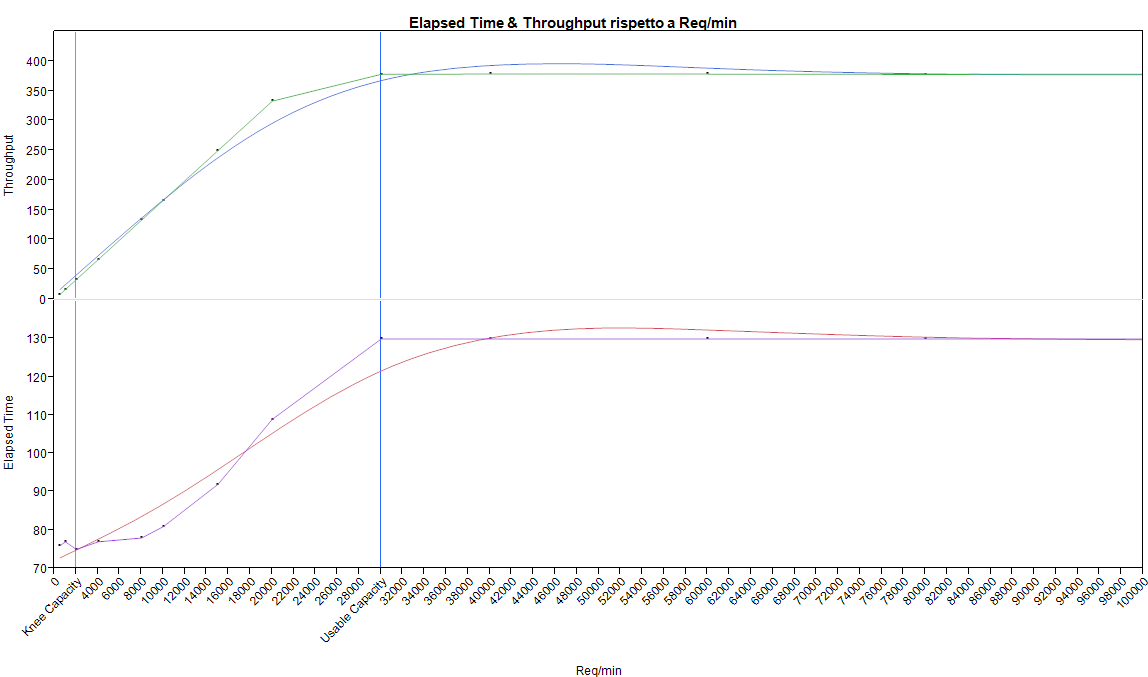
\includegraphics[width=\linewidth, keepaspectratio]{usable_knee_medium}
  \caption{Capacity: Knee (2000 Req/min) / Usable (30000 Req/min)}
\end{figure}

\clearpage

\subsection{Test pagine HTML grandi}
In questo caso sono state utilizzate esclusivamente le richieste HTTP per le pagine
\textit{big\_text} e \textit{big\_image}.\\
In \figurename~\ref{big_page_summary_report} sono presenti gli esiti del
Summary Report di JMeter.\\

\begin{figure}[!htbp]
  \centering
  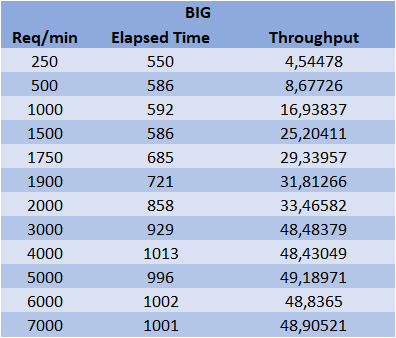
\includegraphics[width=.4\linewidth, keepaspectratio]{capacitytest_big}
  \caption{Test pagine HTML grandi}
  \label{big_page_summary_report}
\end{figure}

Utilizzando il costruttore di Grafici di \textit{JMP} sono stati analizzati i plot
di Throughput ed Elapsed Time, e definiti i punti di \textit{Knee Capacity} e
\textit{Usable Capacity}.\\

\clearpage

\begin{figure}[!htbp]
  \centering
  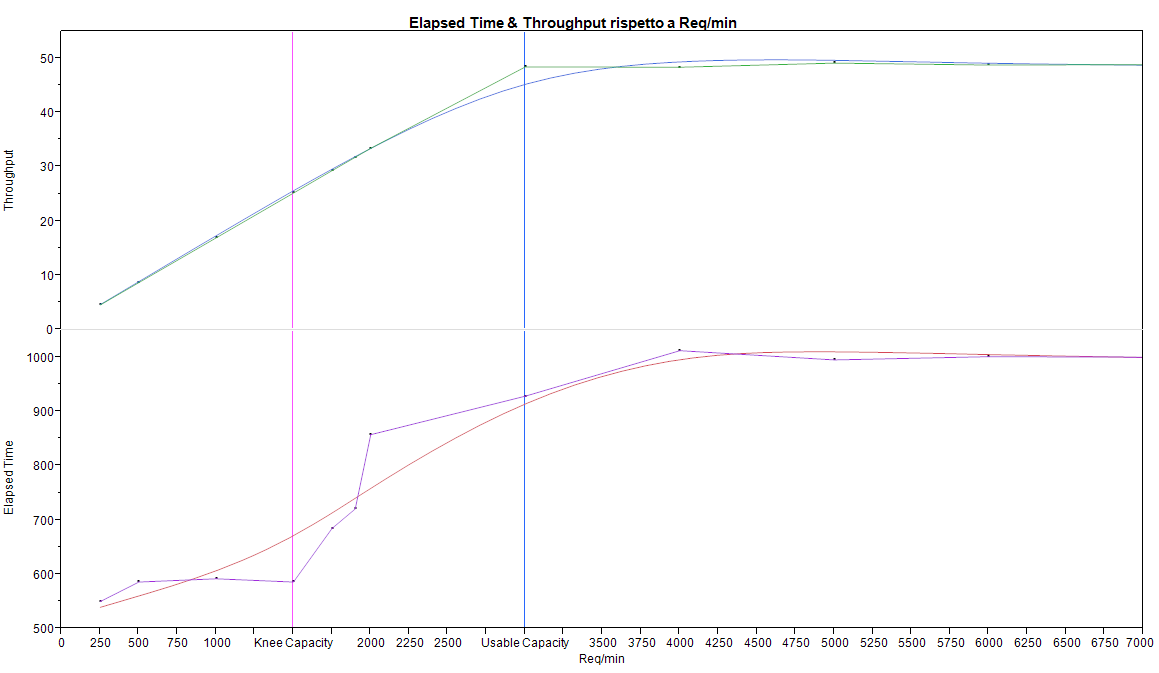
\includegraphics[width=\linewidth, keepaspectratio]{usable_knee_big}
  \caption{Capacity: Knee (1500 Req/min) / Usable (3000 Req/min)}
\end{figure}

\subsection{Test Random}
Finora sono state studiate le capacità di carico del sistema in presenza delle
tre differenti tipologie di pagine HTML disponibili.\\
Dai test effettuati è possibile ricavare il caso medio e il caso peggiore per
ognuno dei punti di funzionamento considerati:
\begin{itemize}
  \item Caso Medio:
  \begin{itemize}
    \item \textbf{Knee Capacity} - 6167
    \item \textbf{Usable Capacity} - 31000
  \end{itemize}
  \item Caso Peggiore:
  \begin{itemize}
    \item \textbf{Knee Capacity} - 1500
    \item \textbf{Usable Capacity} - 3000
  \end{itemize}
\end{itemize}

Come era possibile aspettarsi, il caso peggiore corrisponde esattamente all'uso
delle pagine HTML grandi.\\

Per verificare il reale comportamento del sistema, è stato effettuato un ulteriore
capacity test per definire i punti di funzionamento nel caso di un Random Controller
che genera, in maniera uniforme, richieste HTTP relative a tutte le tipologie di
pagine.\\

In \figurename~\ref{random_page_summary_report} sono presenti gli esiti del
Summary Report di JMeter.\\

\begin{figure}[!htbp]
  \centering
  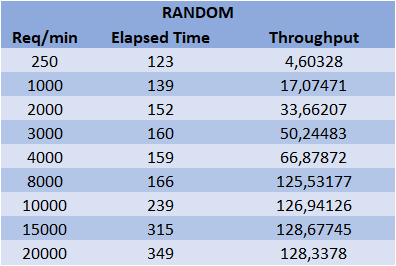
\includegraphics[width=.4\linewidth, keepaspectratio]{capacitytest_random}
  \caption{Test pagine random}
  \label{random_page_summary_report}
\end{figure}

Utilizzando il costruttore di Grafici di \textit{JMP} sono stati analizzati i plot
di Throughput ed Elapsed Time, e definiti i punti di \textit{Knee Capacity} e
\textit{Usable Capacity}.\\

\begin{figure}[!htbp]
  \centering
  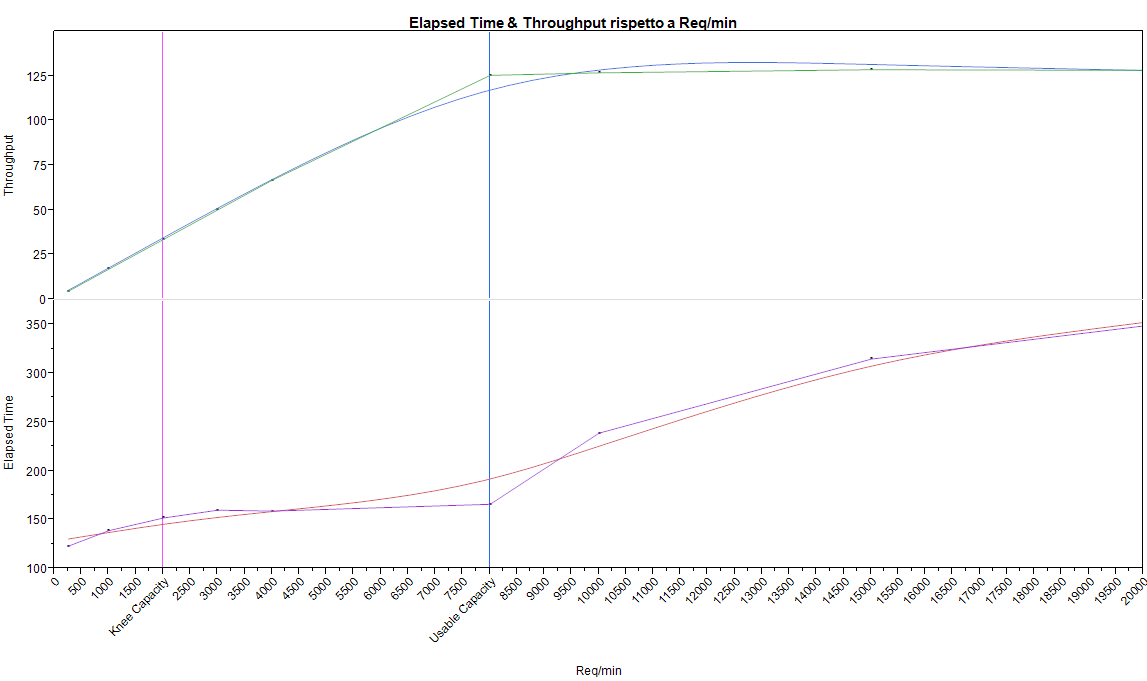
\includegraphics[width=\linewidth, keepaspectratio]{usable_knee_random}
  \caption{Capacity: Knee (2000 Req/min) / Usable (8000 Req/min)}
\end{figure}
